\usetikzlibrary{positioning, fit, shapes.geometric, arrows.meta, shadows, calc}

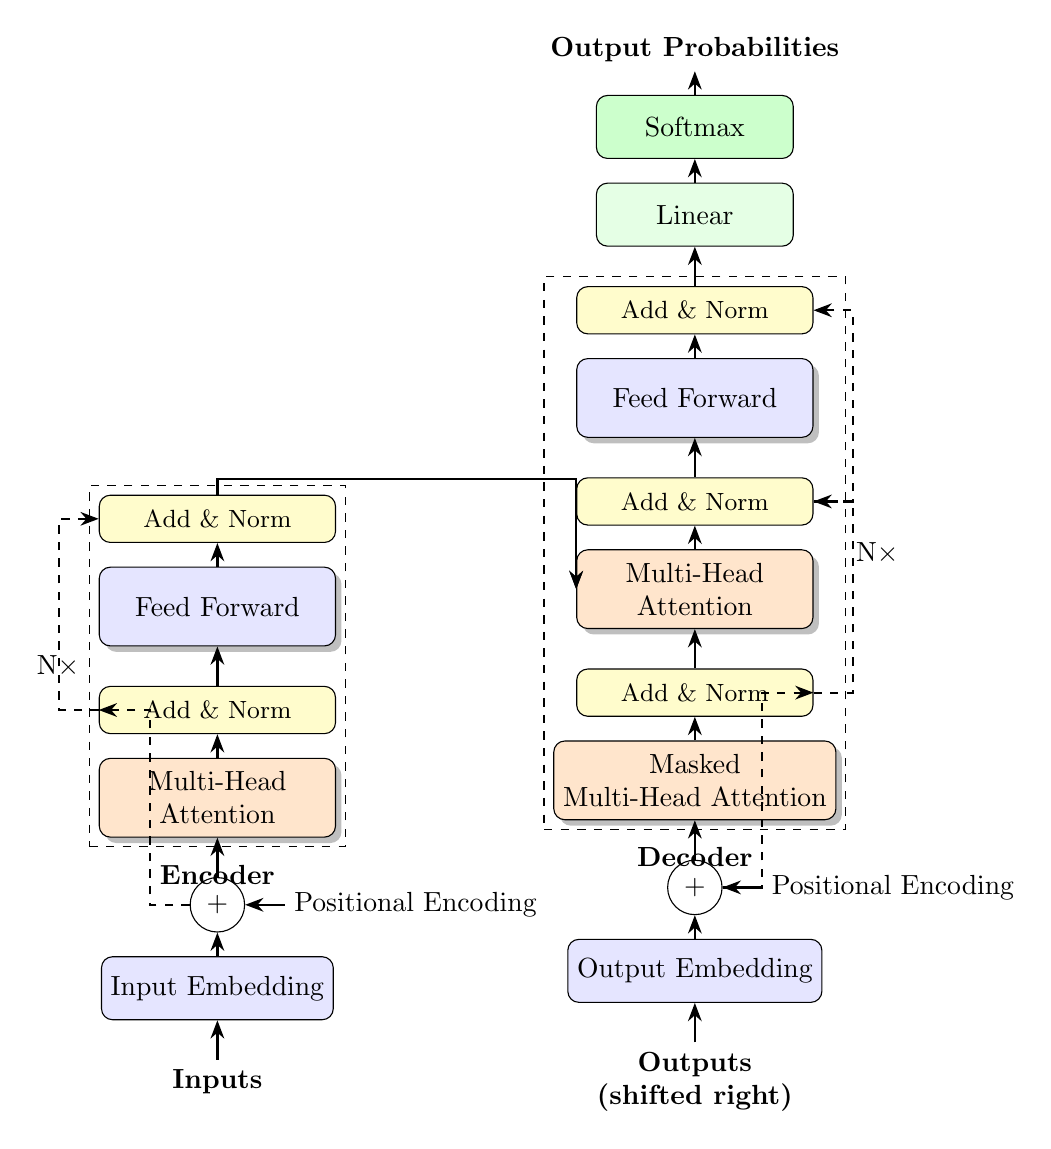
\begin{tikzpicture}[
    node distance=0.8cm and 1cm,
    layer/.style={
        draw,
        rectangle,
        rounded corners,
        minimum width=3cm,
        minimum height=1cm,
        align=center,
        fill=white,
        drop shadow
    },
    process/.style={
        draw,
        rectangle,
        rounded corners,
        minimum width=2.5cm,
        minimum height=0.8cm,
        align=center,
        fill=blue!10
    },
    arrow/.style={
        ->,
        >=Stealth,
        thick
    },
    addnorm/.style={
        draw,
        rectangle,
        rounded corners,
        minimum width=3cm,
        minimum height=0.6cm,
        fill=yellow!20,
        align=center,
        font=\small
    }
]

% Encoder Stack
\node[font=\bfseries] (input) {Inputs};
\node[process, above=0.5cm of input] (emb) {Input Embedding};
\node[circle, draw, fill=white, above=0.3cm of emb] (plus1) {+};
\node[right=0.5cm of plus1] (pos) {Positional Encoding};

\node[layer, fill=orange!20, above=0.5cm of plus1] (mha) {Multi-Head\\Attention};
\node[addnorm, above=0.3cm of mha] (norm1) {Add \& Norm};

\node[layer, fill=blue!10, above=0.5cm of norm1] (ffn) {Feed Forward};
\node[addnorm, above=0.3cm of ffn] (norm2) {Add \& Norm};

% Decoder Stack
\node[right=4cm of input, font=\bfseries, align=center] (output) {Outputs\\(shifted right)};
\node[process, above=0.5cm of output] (outemb) {Output Embedding};
\node[circle, draw, fill=white, above=0.3cm of outemb] (plus2) {+};
\node[right=0.5cm of plus2] (pos2) {Positional Encoding};

\node[layer, fill=orange!20, above=0.5cm of plus2] (mmha) {Masked\\Multi-Head Attention};
\node[addnorm, above=0.3cm of mmha] (norm3) {Add \& Norm};

\node[layer, fill=orange!20, above=0.5cm of norm3] (mha2) {Multi-Head\\Attention};
\node[addnorm, above=0.3cm of mha2] (norm4) {Add \& Norm};

\node[layer, fill=blue!10, above=0.5cm of norm4] (ffn2) {Feed Forward};
\node[addnorm, above=0.3cm of ffn2] (norm5) {Add \& Norm};

\node[process, fill=green!10, above=0.5cm of norm5] (linear) {Linear};
\node[process, fill=green!20, above=0.3cm of linear] (softmax) {Softmax};
\node[above=0.3cm of softmax, font=\bfseries] (probs) {Output Probabilities};

% Connections Encoder
\draw[arrow] (input) -- (emb);
\draw[arrow] (emb) -- (plus1);
\draw[arrow] (pos) -- (plus1);
\draw[arrow] (plus1) -- (mha);
\draw[arrow] (mha) -- (norm1);
\draw[arrow] (norm1) -- (ffn);
\draw[arrow] (ffn) -- (norm2);

% Connections Decoder
\draw[arrow] (output) -- (outemb);
\draw[arrow] (outemb) -- (plus2);
\draw[arrow] (pos2) -- (plus2);
\draw[arrow] (plus2) -- (mmha);
\draw[arrow] (mmha) -- (norm3);
\draw[arrow] (norm3) -- (mha2);
\draw[arrow] (mha2) -- (norm4);
\draw[arrow] (norm4) -- (ffn2);
\draw[arrow] (ffn2) -- (norm5);
\draw[arrow] (norm5) -- (linear);
\draw[arrow] (linear) -- (softmax);
\draw[arrow] (softmax) -- (probs);

% Cross Attention
\draw[arrow] (norm2.north) -- ++(0,0.2) -| (mha2.west);
\draw[arrow] (norm2.north) -- ++(0,0.2) -| (mha2.west); % Simplified, normally K, V

% Residuals (simplified visualization)
\draw[arrow, dashed] (plus1.west) -- ++(-0.5,0) |- (norm1.west);
\draw[arrow, dashed] (norm1.west) -- ++(-0.5,0) |- (norm2.west);

\draw[arrow, dashed] (plus2.east) -- ++(0.5,0) |- (norm3.east);
\draw[arrow, dashed] (norm3.east) -- ++(0.5,0) |- (norm4.east);
\draw[arrow, dashed] (norm4.east) -- ++(0.5,0) |- (norm5.east);

% Labels
\node[draw, dashed, fit=(mha) (norm2), label=left:N$\times$] (enc_block) {};
\node[draw, dashed, fit=(mmha) (norm5), label=right:N$\times$] (dec_block) {};

\node[below=0.1cm of enc_block, font=\bfseries] {Encoder};
\node[below=0.1cm of dec_block, font=\bfseries] {Decoder};

\end{tikzpicture}
